% !TeX root = ../main.tex

\chapter{Device fabrication of silicon nitride ring resonators}

Different from fabrication of silicon-on-insulator, which is CMOS-compatible and fully understood both in the laboratory and semiconductor industry, fabricating integrated silicon nitride device, in particular high Q-factor ring resonators, is only realized in several group all around the word. 

Collaborating with Yokoyama Lab in Kyushu University, we perform the subtractive fabrication of silicon nitride ring resonators, along with other optical devices. To discover the diversity of fabrication recipes and compare the material properties, we also design the device layout and order the devices using ligentec process and NTT-AT process.

\section{Subtractive fabrication process}

The subtractive fabrication of waveguide is widely perform in a variety of material platforms, including silicon nitride. The previous work concerning our fabrication processes reported ring resonators with high \textit{Q}-factor up to \num{5.2d4} and waveguides with measured loss of 2.9 dB/cm \cite{Cheng2017b}. 

\begin{figure}
	\centering
	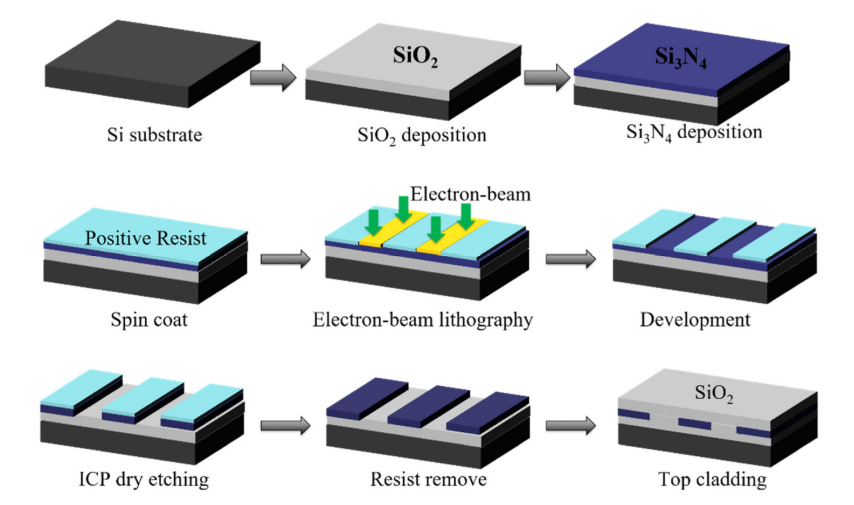
\includegraphics[width=1.0\linewidth]{imgs/png/fab-flow}
	\mycaption{Schematic process flow of the subtractive process}{}
	\label{fig:fab-flow}
\end{figure}

The schematic process flow of the subtractive process is shown in \autoref{fig:fab-flow}. To begin this process, we deposit the silicon dioxide over a 4 inch silicon wafer using the TEOS  (tetraethyl orthosilicate) source or begin with a thermal oxidized wafer. Next step is to deposit silicon nitride film with chemical vapor deposition method. After patternning the layout with electron beam lithography, the silicon nitride layer is etched. Following the resist removal, another layer of silica is cladded. Finally, the chip is diced to couple the light from the edge. The details of each step will be explained in the following contents.

%Recently, Si3N4 has been widely utilized in integrated optic devices because of its conspicuous flexibility in the refractive index around 2.0. In our fabrication (Fig. 1), the Si3N4 films with controlled thickness and refractive index were deposited onto the SiO2/Si substrate through LSCVD using the liquid SiN-X source (SAMCO Inc.) with N2 or N2O. The measured refractive index of the deposited Si3N4 film was 1.99, which can be turned to between 1.66 and 1.78 as silicon oxynitride (SiOxNy) by mixing N2O gas. The propagation loss of the films also demonstrated a temperature dependence of the deposition. If the temperature is set too low, the chemical reaction may be uncompleted to form Si3N4. We found that the optimal deposition temperature was 150C to obtain the required low loss properties. The photonic patterns of waveguides, ring resonators, and grating couplers were transferred onto the resist layer on Si3N4 by using the electron beam lithography (EBL) technique. The direct write capability of EBL guarantees the small feature size and high accuracy of the device. After development, the patterned resist was hard-baked at 150C for 5 minutes. This process is effective to improve the dry etching selectivity of the resist and Si3N4, and to help to achieve rectangle waveguide cross-sections. We used a mixed gas of CHF3/O2 for the inductively coupled plasma reactive ion etching (ICP-RIE). After etching to reach the desired depths, we striped the leftover resist using the RIE in which the O2 plasma removes only the resist, but leaves the exposed Si3N4 waveguide untouched. By utilizing CVD, we deposited a top cladding of SiO2 onto the Si3N4 core to form a buried ridge waveguide resonator

\subsection{Film deposition}

The traditional method to grow silicon nitride is using low pressure CVD (LP-CVD) method. The silicon source is usually silane (\ce{SiH4}) or chloride silane, such as dichlorosilane (DCS, \ce{SiH2Cl2}), which is vapor phase and toxic \cite{Kaloyeros2017}, while the ammonia gas (\ce{NH3}) plays the role of nitrogen source. An alternative approach is using modern plasma-enhanced CVD (PE-CVD) with liquid source, which has faster growing rate and lower reaction temperature.

Although the silicon nitride waveguides deposited by LP-CVD method are mainly reported, it is necessary to figure out the CVD method dependence of film properties, especially the refractive index. 

% Except the difference of precursors, the silicon nitride formation and deposition techniques can influence the film properties. The plasma-enhanced CVD (PE-CVD) is one alternative which has faster growing rate and lower reaction temperature. Based on PE-CVD, liquid source CVD is developed in several industry sectors.

In our research, we choose three different CVD facilities---LP-CVD, PE-CVD and liquid source CVD as the film deposition facilities, and adopt different recipes to deposit the silicon nitride layer. Compared with commercial LP-CVD silicon nitride wafers,
the details of PE-CVD and LS-CVD recipes are listed in \autoref{tab:cvd}. It is apparent from the data that LS-CVD has the fastest rate and lowest reaction temperature. In addition, although the flow rate of SN-2 source changes the film growing rate 23 nm/min, it does not effect on the film stoichiometry and optical properties. This is different from PE-CVD facility used in this research, which can be also used to produce silicon-rich or nitrogen-rich films as controlling the gas ratio.
It is worth to mention that all the wafer deposited with above three recipes shows no cracks during the fabrication, suggesting low tensile in silicon nitride films.

\begin{table}[]
\centering
\begin{tabular}{cccc}
\hline
              & LP-CVD                            & PE-CVD                                                                                  & LS-CVD                                                                                  \\ \hline
Facility      & -                                 & SAMCO PD-220NL                                                                          & SMACO PD-100ST                                                                          \\ \hline
Source        & DCS:NH3:N2                        & \begin{tabular}[c]{@{}c@{}}\ce{SiH4}:\ce{NH3}:N2\\ =6:5:189 sccm\end{tabular}                     & \begin{tabular}[c]{@{}c@{}}SN-2:\ce{N2}\\ =0.5:30 sccm\end{tabular}                          \\ \hline
Chamber Temp. & 750\si{\celsius}-800\si{\celsius} & \begin{tabular}[c]{@{}c@{}}upper 150\si{\celsius}\\ lower 350\si{\celsius}\end{tabular} & \begin{tabular}[c]{@{}c@{}}upper 150\si{\celsius}\\ lower 180\si{\celsius}\end{tabular} \\ \hline
RF Power      & -                                 & 40 W                                                                                     & 30 W                                                                                     \\ \hline
Deposition Rate          & -                                 & 15 nm/min                                                                               & 23 nm/min                                                                               \\ \hline
\end{tabular}
\mycaption{Recipes of CVD methods used in this research}{In the case of PE-CVD and LS-CVD, upper electrode and lower electrode are set at different temperature. RF power refers to radio frequency power used to excite the precursor gasses.}
\label{tab:cvd}
\end{table}


\subsection{Material properties}
The vast majority of studies concerning silicon nitride processes have found that the hydrogen remaining in the film leads to N-H and Si-H bond, which influence the absorption at S and C band \cites{Ay2004, Agnihotri2000}. 

To quantitatively clarify these bonds in the films deposited with CVD facilities mention above, we perform the Fourier-transform infrared spectroscopy on the surface silicon nitride film. The absorbance is taken from the difference with background, From \autoref{fig:ftir}, it can be seen that except the peak around 870 \si{\per\cm}, two other peaks are located around 2200 and 3300 \si{\per\cm}, corresponding to Si-H and N-H bonds respectively.

Interestingly, there are also two peaks found at ? and ?, indicating Si-O symmetric and asymmetric stretching bonds respectively. This result may be explained by the fact that the infrared 



\cite{Shaw2005}

\begin{figure}
    \centering
    \includesvg{ftir}
    \caption{Caption}
    \label{fig:ftir}
\end{figure}

\subsection{Patterning and etching}

\subsection{Top-cladding and annealing}

\subsection{Optical I/O and packaging}

\section{Fabless samples via foundries}

\subsection{Ligentec}

\subsection{NTT-AT}

